\chapter{Introduction}
Computer vision applications on handheld devices is an area which has received growing interest in recent years. 
Modern smartphones are cheap, and their cameras and CPUs are good enough for many computer vision purposes.
% TODO hitta källa som säger nåt intressant om detta

An interesting computer vision problem which can be useful to solve with a smartphone, is to measure the dimensions of an object, a cuboid package for example.
Imagine that one would like to know the dimensions of a package, but does not have a measuring tool.
Since almost everyone carries a smartphone with them, a practical solution would be to have an application on one's smartphone which can measure the package, without measuring tape or ruler.
If a reference object, like a credit card for example, is placed on top of the package, it could be possible to measure its dimensions by filming the package and reference object together.

\section{Requirements} \label{introduction:requirements}
In order for a measuring solution like the one described above to be useful, it must be easy to use. 
The measuring process should therefore not require any user intervention, such as marking the reference object or package in the image. 
They need to be \textit{detected automatically} by the application.

Computer vision applications which aim to extract metric information from a scene typically require knowledge about the internal properties and pose of the camera.
The most standard way to gather this information is to perform a calibration procedure in advance, by observing a known calibration object, e.g. a printed paper with a special pattern on it.
In this scenario, a preparation step like this is very undesirable from a user perspective, it would probably be more convenient to measure the package manually.
Therefore, gathering the necessary information cannot not require any additional steps, such as calibrating the camera manually.
In other words, the problem must be solved using an \textit{uncalibrated view}.

A measuring application must not only be easy to use, it must also have good performance.
Performance can be broken down to three key aspects: robustness, accuracy and speed.
Robustness is defined as the success rate of the method, i.e. the rate at which an adequately correct result is achieved.
Accuracy is defined as the average precision of the result when a correct result is achieved.
Speed refers to the average processing time.

The ultimate goal with regard to speed is to reach real time performance, i.e. processing times of less than 30-40 milliseconds per frame \cite{pulli2012real}.
This is a challenging goal, especially with the limited processing power of a mobile device.
However, in this case it is considered more important that the method is accurate and robust, short processing times are a secondary goal.
Still, as a step to reduce processing time, and to reduce the computational complexity of the method, only a single image will be used at a time, as opposed to analysing multiple images and before delivering an answer.
In other words, the problem will be solved using a \textit{single uncalibrated view}.

\section{Problem statement}\label{problem-statement}
The goal of this thesis is to implement and evaluate a method to automatically measure the dimensions of cuboid packages with a mobile device, using a single uncalibrated view.
This will be done by placing a known reference object on top of the package, and filming the package and reference object together.
The package and reference object will be detected and localised automatically by the application, after which the dimensions of the package are calculated.

Detection and localisation are to be performed with a model-based detector.
The detector will use the edge information in the image to detect and localise the objects.
A model-based detector is used for simplicity, and because it is deemed appropriate because cuboid packages have a well-defined shape which should be easy to detect with edge data.

Uncalibrated measurements will be achieved by using the geometric properties of cuboids to determine the internal parameters of the camera. More specifically, the vanishing points formed by the edges of the package will be used.

Every cuboid package give rise to three orthogonal vanishing points when viewed in a perspective image, as shown in figure \ref{fig:vanishing_points}.
Using vanishing points to determine the internal parameters of a camera is called "vanishing point calibration", and it is described further in section \ref{related_work:vanishing_point_calibration} and \ref{camera-calibration}.

In general, vanishing point calibration can be problematic, since it is not always be possible to find three orthogonal vanishing points in an image, and they can be difficult to find automatically even if present.
In this case however, it is ideal, since every cuboid package has three orthogonal faces.
Additionally, the edges which give rise to the vanishing points must be found in order to measure the package regardless of calibration method, so detecting the vanishing points requires no extra work.

\begin{figure}
\begin{center}
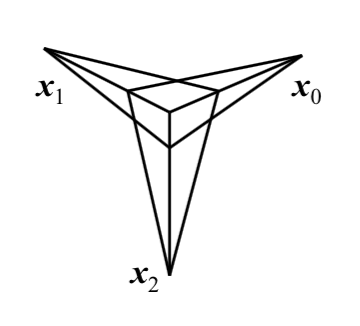
\includegraphics[width=0.6\textwidth]{figures/vanishing_points.png}
\end{center}
\caption{Visualisation of how the edges of a cuboid give rise to three orthogonal vanishing points: $x_0$, $x_1$, and $x_2$.} % TODO hur referera? Tagen från szeliski s. 330
\label{fig:vanishing_points}
\end{figure}

While using an uncalibrated view is more convenient, a calibrated view is expected to yield higher accuracy.
If so, it would be interesting to know how much accuracy needs to be sacrificed to gain the extra utility of not needing prior calibration.
In order to determine this, a version which uses a calibrated view will also be implemented.
The calibrated version will serve as a baseline implementation, to which the performance of the uncalibrated method will be compared.

For this approach to be successful, two components must exist, and work well: a detection component and a measuring component.
The detection component should find the position of the reference object and the package in the image, and the measuring component should use their positions to calculate the dimensions of the package.

To assess the quality of the result, the two components will be evaluated by measuring success rate and accuracy.
Success rate is defined as the rate at which the result is reasonably correct.
Accuracy is defined as how accurate the result is when a correct solution is found.
The components will both be evaluated in isolation, and combined.

In principle all of the above can be tested offline, using pictures taken with a smartphone.
This will be the primary method used when evaluating the result.
However, since the purpose of the program is to be used in a smartphone, it will also be embedded in a smartphone demo app, to show that it performs well enough in its intended environment and that the program is fast enough to be used in a smartphone.

\section{Purpose} 
The main scientific purpose of this thesis is to determine the feasibility of an automatic cuboid measurer on a handheld device.
This specific setting provides several interesting challenges.
The application must have high accuracy, robustness, and speed in order to be useful.
The method used to solve the problem must require minimal effort from the user, which is why detection of the reference object and package is to be automatic, and camera calibration is to be avoided.
Camera calibration is to be avoided by exploiting the geometry of cuboids to find vanishing points which can be used to calibrate the camera automatically.
This fact provides another scientific purpose: to determine whether or not it is feasible to use vanishing point calibration to measure the dimensions of cuboids from a single image.

While it is certain that the camera can be calibrated with three orthogonal vanishing points, it is not clear if the result will be accurate enough to make good measurements \cite[195-226]{hartley-zisserman}.
As presented further in section \ref{related_work:vanishing_point_calibration} the related work uses either multiple views or a large amount of lines in the image to find the vanishing points.
Here, maximum three lines will contribute to each vanishing point in a single image, which may reduce accuracy.

\section{Delimitations}
In a finished consumer smartphone application, it would be desirable to have the option to choose between a multitude of reference objects, like credit cards, matchboxes, smartphones, papers, and more. 
To simplify the detection component, only white papers from the ISO 216 A-series (e.g. A4 or A5) will be considered as reference objects in this thesis.
The reason behind this choice is that papers of this type are very common, and should be easy to detect.

The type of packages considered are limited to packages with a cuboid shape, and with a colour that has reasonable contrast to that of the reference object. The package must stand on a flat surface, and the area in close proximity to the package should be empty.

% TODO Section about Bontouch/Postnord???
